\noindent This topic covers results of Bogoliubov, Parasiuk, Hepp, Zimmermann, or the BPHZ renormalization scheme. \\

\noindent A \textit{renormalizable} theory is a cutoff field theory determined by a finite number of parameters $\hat{H}_\Lambda = \hat{H} (z_1, \dots, z_n; \Lambda)$ such that for all observables $\hat{A}_\alpha$, the expectation value of $\hat{A}$ can be matched to experimentally determinable quantities for any choice of cutoff $\Lambda$ by redefining the parameters $z_j = z_j (\Lambda)$

\begin{equation}
\langle \hat{A}_\alpha \rangle _{z_1, \dots, z_n, \Lambda} = \langle \hat{A}_\alpha \rangle _{z_1 (\Lambda), \dots, z_n (\Lambda)} = \text{Experiment} (\alpha) .
\end{equation}

\noindent There is a weak form of renormailzability that retains dependence of the expectation value on the cutoff

\begin{equation}
\langle \hat{A}_\alpha \rangle _{z_1 (\Lambda), \dots, z_n (\Lambda)} = \text{Experiment} (\alpha) + \mathcal{O} \left(\frac{1}{k_c}\right).
\end{equation}

\noindent This dependence can be worked around, since as $k_c \rightarrow \infty$, the inverse goes to zero. \\

\noindent In the $\phi^4$ interaction, we have three parameters with the Hamiltonian

\begin{equation}
\hat{H} (m, \lambda, z ; \Lambda)
\end{equation}

\noindent Where $z$ is the field strength renormalization parameter. \\

\noindent Is $\phi^4$ theory, by this definition, renormalizable? \\

\noindent If this is true, then we are allowed to fit an infinite number of quantities to experimentally determinable quantities by fitting only three parameters: $m$, $\lambda$, and $z$. Very cool! \\

\subsection*{Degree of Divergence}

\noindent Consider a diagram with $B_E$ external lines. The diagram has a \textit{superficial degree of divergence} $D$ if it diverges with the cutoff as $k_c^D$. For $D=0$, we say that the diagram has logarithmic divergence: $\log{(k_c)}$. \\

\noindent \textbf{Theorem}: The degree of divergence is equal to the number of spacetime dimensions minus the number of external lines

\begin{equation}
D = 4 - B_E .
\end{equation}

\textbf{Examples}:

\begin{figure}[H]
	\centering
	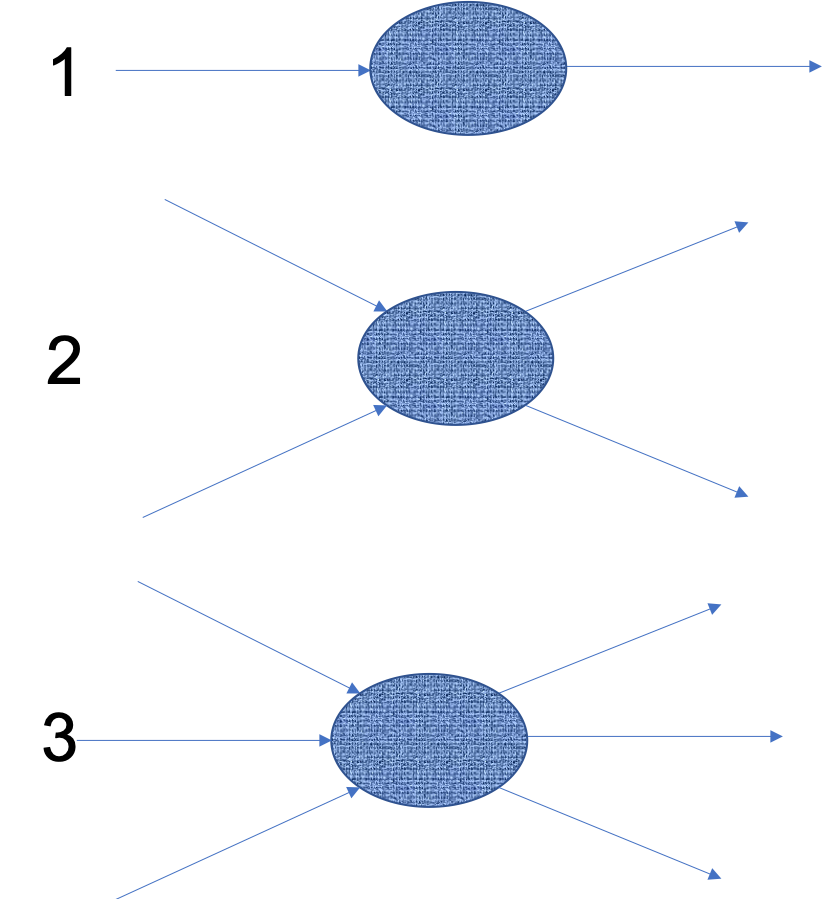
\includegraphics[width=2in]{images/dod_ex1.png}
\end{figure}

\begin{enumerate}
\item $B_E = 2 \implies D = 2 \implies \sim k_c^2$
\item $B_E = 4 \implies D = 0 \implies \sim \log{(k_c)}$
\item $B_E = 6 \implies D = -2 \implies \sim \frac{1}{k_c^2}$
\end{enumerate}

\noindent Note that as $B_E$ and $k_c$ increase, the divergences become increasingly less observable. Each pair of incoming/outgoing particles contributes a propagator proportional to $k_c^{-2}$ to the $4D$ momentum integral $\sim \,\, \int \frac{d^4 k}{(2 \pi)^4} \, \left(\frac{i}{k^2 - m^2 + i \epsilon}\right)^{\frac{B_E}{2}}$.  \\

\noindent Some more notation: $B_I$ is the number of internal lines, $V$ is the number of vertices, and $L$ is the number of closed loops. \\

\begin{figure}[H]
	\centering
	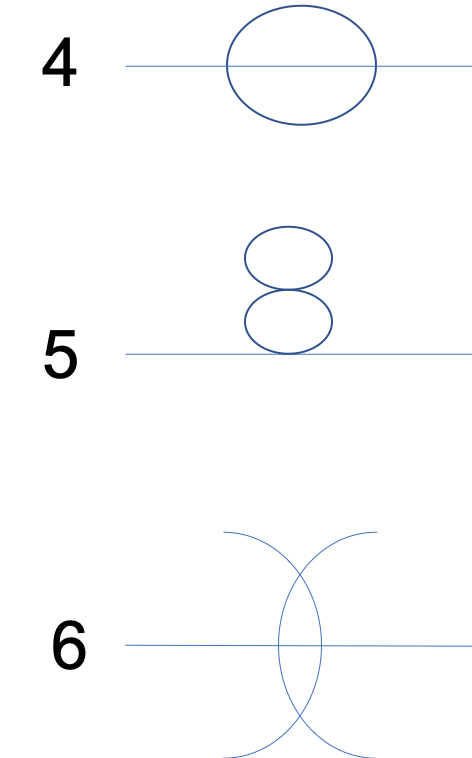
\includegraphics[width=1.5in]{images/dod_ex2.png}
\end{figure}

\begin{enumerate}
\item $B_I = 3$, $V=2$, $L=2$, $D=2$
\item $B_I = 3$, $V=2$, $L=2$, $D=2$
\item $B_I = 5$, $V=4$, $L=2$, $D=-2$
\end{enumerate}

\noindent \textbf{Proof}: \\

\noindent The number of loops corresponds directly to the number of undetermined momenta ($4D$ momentum space integrals). Morally, we say that $\int \frac{d^4 k}{(2 \pi)^4} \sim k_c^4$. \\
 
 \noindent It seems that there are $B_I$ such integrals, but momentum conservation reduces the total number of loop integrals to 
 
\begin{equation}
L = B_I - (V - 1).
\end{equation}

\noindent Each vertex has four lines and each line connects two vertices, such that 

\begin{equation}
4V = B_E + 2 B_I.
\end{equation}

\noindent Now, recall that for each loop there is a factor $\sim k_c^4$ from the integral, and for each line there is a factor $k_c^{-2}$ from the propagator. Then

\begin{equation}
D = 4 L - 2 B_I = 4 - B_E .
\end{equation}

\noindent \textbf{Exercise}: Prove this result for $n$-dimensional spacetime.

\subsection*{Physical or Renormalized Perturbation Theory}

\noindent Consider the parameterized Lagrangian

\begin{equation}
\mathcal{L} = \mathcal{L} (z_1 = m, z_2 = \lambda, z_3 = z) = \frac{1}{2} (z^2 (\partial_\mu \phi)^2 - z^2 m^2 \phi^2 ) - z^4 \frac{\lambda}{4!} \phi^4.
\end{equation}

\noindent Rewrite this in terms of the physical Lagrangian, the one that has been successful in corresponding with experimental data, and counter terms dependent on three new parameters $A$, $B$, and $C$,

\begin{align}
\mathcal{L} &= \mathcal{L}_{\text{phys}} + \text{counter terms} \\
\mathcal{L} &= \left(\frac{1}{2} (z^2 (\partial_\mu \phi)^2 - m_{\text{phys}}^2 \phi^2 ) - z^4 \frac{\lambda_{\text{phys}}}{4!} \phi^4 \right) + \left( A (\partial_\mu \phi )^2 + B \phi^2 + C \phi^4  \right)
\end{align}

\noindent Now, think of these parameters as additional interactions that can be shifted to eliminate the dependence on the cutoff. These parameters are determined iteratively by the constraint that physically observable quantities do not depend of the momenta $k$. \\

\noindent The Feynman rules for the renormalized $\phi^4$ theory are the same rules plus two more due to an additional type of vertex that depend of the ``additional interaction'' parameters.

\begin{figure}[H]
	\centering
	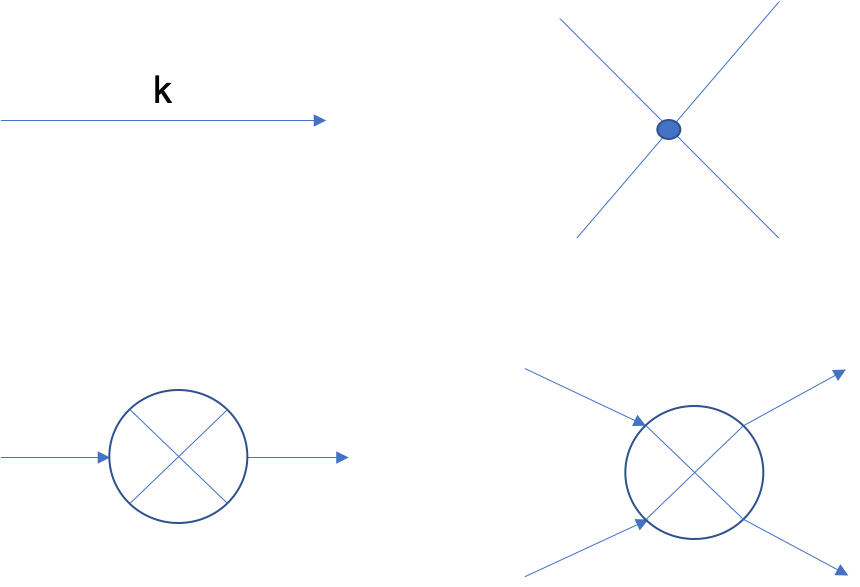
\includegraphics[width=3in]{images/renorm_feynman.png}
\end{figure}

$$
\begin{array}{lc}
\text{Top-left:} & \frac{i}{k^2 - m_{\text{phys}}^2 + i \epsilon} \\
\text{Top-right: }& -i \lambda_{\text{phys}} \\
\text{Bottom-left:} & 2 i (A k^2 + B) \\
\text{Bottom-right:} & 4! \cdot i C
\end{array}
$$

\noindent So, counter terms are added to the Lagrangian as ``additional interactions'', which introduce new Feynman diagrams. The parameters are determined iteratively to order $\lambda_{\text{phys}}^N$, at which we call them $A_N$, $B_N$, and $C_N$, and nothing depends on the cutoff. \\

\noindent The next iteration $N+1$ is determined by requiring that the new propagator (bottom-left diagram above) at $\lambda_{\text{phys}}^{N+1}$ has a pole at $m_{\text{phys}}$ with residue equal to one. We also require that the scattering amplitude to order $\mathcal{O} (\lambda_{\text{phys}}^{N+1})$ is equal to $-i \lambda_{\text{phys}}$ (bottom-right diagram above). \\

\subsection*{Non-Renormalizable Theories}

\noindent A non-renormalizable theory requires an infinite number of parameters to ensure that operationally-defined quantities do not depend on the cutoff. \\

\noindent How do these theories appear in renormalized perturbation theory? \\

\noindent For instance, consider the Lagrangian

\begin{equation}
\mathcal{L} = \mathcal{L}^0_{\text{phys}} + \mathcal{L}^{int}_{\text{phys}} (\lambda) + (\text{counter terms}) .
\end{equation}

\noindent Calculate the scattering amplitude to order $\mathcal{O} (\lambda_{\text{phys}}^{N})$, and we will see that we need counter terms to eliminate dependence on the cutoff $k_c$, but as we go to higher and higher order in $\lambda_{\text{phys}}$, we need more and more counter terms, and this will continue and diverge, requiring an infinite number of counter terms and associated parameters to eliminate the cutoff dependence.